\documentclass[12pt,a4paper]{../krautsourcing/homework}
\usepackage[utf8]{inputenc}
\usepackage[ngerman]{babel}
\usepackage[T1]{fontenc}
\usepackage{amsmath}
\usepackage{graphicx}
\usepackage{amsfonts}
\usepackage{amssymb}
\usepackage{lmodern}
\usepackage{amsmath}
\usepackage{amssymb}
\usepackage{paralist}
\usepackage{tabularx}
\usepackage{tikz}
\usetikzlibrary{automata,positioning,backgrounds,calc}

\author{Ruben Felgenhauer,\\Alexander Hildebrandt,\\Leonhard Reichenbach}
\datef{14}{12}{2015}
%\date{\today}
\course{Formale Grundlagen der Informatik II}
\sheet{9}
\sectionprefix{Übungsaufgabe \thesheet.}
\subsectionprefix{\thesheet.}
\subsubsectioncounter{\alph{subsubsection}}
\group{06}
\subsubsectionprefix{(}
\subsubsectionsuffix{)}

\begin{document}

\makeheadline

\addtocounter{section}{2}

\section{}

\subsection{}

\begin{align*}
B = 
\left\lbrace \begin{pmatrix}
0\\0\\0\\3\\2\\0
\end{pmatrix},
\begin{pmatrix}
0\\0\\0\\3\\0\\2
\end{pmatrix},
\begin{pmatrix}
0\\0\\0\\3\\1\\1
\end{pmatrix} \right\rbrace
\end{align*}

In dem Netz \(N_{9.3}\) können im oberen Abschnitt und von der Transition \(c\) Marken erzeugt werden. \(c\) kann jedoch schon mit insgesamt 5 Marken unendlich oft geschaltet werden, dies ist im oberen Abschnitt nicht möglich. Damit \(c\) unendlich oft schalten kann werden 3 Marken in \(p_3\) und 2 Marken in \(p_4\) benötigt. Da die Marken von \(p_5\) nach \(p_4\) geschaltet werden können ergeben sich die obigen drei Anfangsmarkierungen.

\subsection{}

\centerline{
\begin{tikzpicture}[auto, baseline, node distance=20mm]
\node[initial,initial text={}] (42011) {\((4,2,0,1,1)^T\)};
\node[below=of 42011]          (42020) {\((4,2,0,2,0)^T\)};
\node[right=of 42020]          (1w020) {\((1,\omega,0,2,0)^T\)};
\node[right=of 1w020]          (www20) {\((\omega,\omega,\omega,2,0)^T\)};
\node[right=of www20]          (wwww0) {\((\omega,\omega,\omega,\omega,0)^T\)};
\node[at=(1w020|-42011)]       (1w011) {\((1,\omega,0,1,1)^T\)};
\node[at=(www20|-42011)]       (www11) {\((\omega,\omega,\omega,1,1)^T\)};
\path[->,shorten <=1mm, shorten >=1mm]
    (42011) edge             node[above] {\(a\)}   (1w011)
    (42011) edge             node[left]  {\(d\)}   (42020)
    (42020) edge             node[below] {\(a\)}   (1w020)
    (1w020) edge             node[below] {\(b\)}   (www20)
    (www20) edge             node[below] {\(c\)}   (wwww0)
    (www20) edge[loop below] node[below] {\(a,b\)} ()
    (wwww0) edge[loop below] node[below] {\(c\)}   ()
    (1w011) edge             node[left]  {\(d\)}   (1w020)
    (1w011) edge             node[above] {\(b\)}   (www11)
    (www11) edge             node[left]  {\(d\)}   (www20)
    (www11) edge[loop above] node[above] {\(a,b\)} ()
; %-path-%
\end{tikzpicture}
}

\vspace{5mm}

\stepcounter{section}
\section{}

\subsection{}

Wir ermitteln die Wirkungsmatrix \(\Delta\), die P-Invariantenvektoren \(i_k\) und die T-Invariantenvektoren \(j_k\):
\begin{align*}
    \Delta = \left( \begin{array}{c|cccccc}
        & t1 & t2 & t3 & t & t5 & t6 \\
        \hline
        pa & -1 & 0 & 1 & -1 & 0 & 1\\
        pp & 0 & -1 & 1 & 0 & -4 & 4\\
        p1 & 1 & -1 & 0 & 0 & 0 & 0\\
        p2 & 0 & 1 & -1 & 0 & 0 & 0\\
        p3 & 0 & 0 & 0 & 1 & -1 & 0\\
        p4 & 0 & 0 & 0 & 0 & 1 & -1
    \end{array} \right)
	; \quad
	j_{1} = \begin{pmatrix}
	1 \\ 1 \\ 1 \\ 0 \\0 \\0
	\end{pmatrix}
	;\quad
	j_{2} = \begin{pmatrix}
	0 \\ 0 \\ 0 \\ 1 \\1 \\1
	\end{pmatrix}
	; \quad
	i_1 = \begin{pmatrix}
	0\\1\\0\\1\\0\\4
	\end{pmatrix}
	; \quad
	i_2 = \begin{pmatrix}
	4\\-1\\4\\3\\4\\0
	\end{pmatrix}
\end{align*}

\begin{align*}
	\Delta \cdot j_1 \ = \ \Delta \cdot j_2 \ = \ \Delta^T \cdot i_1 \ = \ \Delta^T \cdot i_2 \ = \ 0
\end{align*}

\subsection{}

Die Menge \(I\) der P-Invarianten des Netzes lautet:
\begin{align*}
    I &= \text{kern}(\Delta^T) \setminus \{0\}\\ &= \text{span}\{(e,d+e,c+e,b+e,a-b,a,a-b+c,a-b+d,d,c,b)^T \mid a,b,c,d,e \in \mathbb{N}_+ \}
\end{align*}

\stepcounter{subsection}

\subsection{}

\begin{align*}
   \Delta = \left( \begin{array}{c|cccccc}
       & a & b & c & d & e & f \\
       \hline
       p1 &  1 & -1 &  0 &  0 &  0 &  0 \\
       p2 &  0 &  0 &  1 & -1 &  0 &  0 \\
       p3 &  0 &  0 & -2 &  2 &  0 &  0 \\
       p4 &  0 &  0 &  0 &  0 & -1 &  1 \\
       p5 &  0 &  1 &  0 &  0 & -1 &  0 \\	
   \end{array}\right)
\end{align*}

\subsection{}

Die Menge \(I\) der P-Invarianten des Netzes lautet:
\begin{align*}
    I = \text{kern}(\Delta^T) \setminus \{0\} = \text{span}\{(0,-2,-1,0,0)^T\} = \{(0,2a,a,0,0)^T \mid a \in \mathbb{N}_+ \}
\end{align*}

\subsection{}

\centerline{
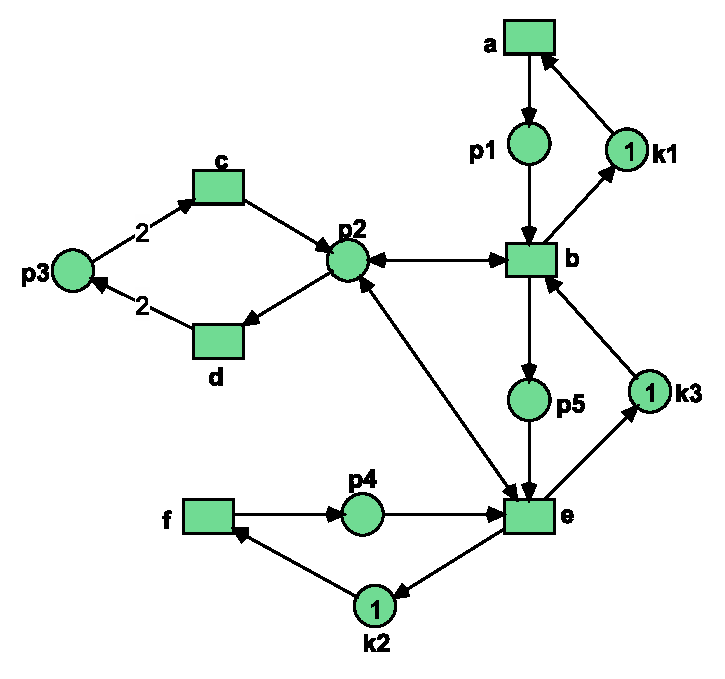
\includegraphics[scale=0.8]{aufgabe-9-5-6.pdf}
}

\begin{align*}
   \Delta' = \left( \begin{array}{c|cccccc}
       & a & b & c & d & e & f \\
       \hline
       p1 &  1 & -1 &  0 &  0 &  0 &  0 \\
       p2 &  0 &  0 &  1 & -1 &  0 &  0 \\
       p3 &  0 &  0 & -2 &  2 &  0 &  0 \\
       p4 &  0 &  0 &  0 &  0 & -1 &  1 \\
       p5 &  0 &  1 &  0 &  0 & -1 &  0 \\	
       k1 & -1 &  1 &  0 &  0 &  0 &  0 \\
       k2 &  0 &  0 &  0 &  0 &  1 & -1 \\
       k3 &  0 & -1 &  0 &  0 & -1 &  0 \\
   \end{array}\right)
\end{align*}
\begin{align*}
    I' &= \text{span}\{(1,0,0,0,0,1,0,0)^T,(0,2,1,0,0,0,0,0)^T,(0,0,0,1,0,0,1,0)^T\}
    \\ &= \{(a,2b,b,c,0,a,c,0)^T \mid a,b,c \in \mathbb{N}_+\}
\end{align*}
Wie man sieht, sind alle P-Invarianten echt größer Null, damit ist das Netz strukturell beschränkt.

\subsection{}

\begin{align*}
    \forall \mathbf{m} \in R(\mathcal{N}_{9.4b}) \ : \ 4 p_1 + 2 p_2 + p_3 + p_4 + p_5 + 4 p_6 + p_7 + p_8 = 54
\end{align*}

\end{document}